\chapter[Sensoriamento]{Sensoriamento}

A produtividade de uma cultura pode ser ampliada a partir do controle das mais diversas variáveis do ambiente. O conhecimento de tais parâmetros possibilita ao produtor, a medida do possível, criar as condições que mais favoreçam o desenvolvimento da plantação. As estações desenvolvidas no projeto RICC serão capazes de medir as seguintes grandezas:

	\begin{itemize}
		\item Referentes ao ambiente externo:
		\begin{enumerate}
			\item Umidade
			\item Temperatura
			\item Velocidade e direção do vento
			\item Radiação solar (UV)
			\item Pluviosidade
		\end{enumerate}	 		
	
		\item Referentes ao solo:	
		\begin{enumerate}
			\item Umidade
			\item pH
			\item Temperatura
		\end{enumerate}
		
		\item Referentes a localização
		\begin{enumerate}
			\item GPS
			\item Bússola
		\end{enumerate}	 		
	\end{itemize}
	
	Os dados coletados para o ambiente externo são de extrema importância para a agricultura, pois permitem a modelagem do processo de evapotranspiração, o que caracteriza os ciclos de água e de energia do ecossistema, além de contribuir para a análise e previsão das condições climáticas \cite{perry2009increasing}. Informações sobre o comportamento desse processo na plantação, em conjunto com as características climáticas locais, podem embasar tomadas de decisões agrícolas como: a escolha do período para cultivo, colheita ou plantação \cite{frisvold2013use}; a gestão do processo de irrigação \cite{gowda2008mapping}; antecipação de condições erráticas do clima \cite{gommes2010guide}.
	
	As medições internas do solo fornecem informações mais específicas sobre o estado da plantação e o seu desenvolvimento. Por exemplo, a temperatura do solo tem impacto no processo de germinação das plantas, afetando sua aquisição de nutrientes e absorção de água \cite{bib_sen_01_jose}. Em relação à medição de pH, a maior parte dos solos disponíveis para agricultura no Brasil possuem pH abaixo de 5,5 e isso deve ser monitorado. Um solo ácido pode reduzir a produtividade da plantação, pois afeta a atividade de micro-organismos e a solubilidade de nutrientes importantes para o desenvolvimento das plantas \cite{bib_sen_04_veloso}.. 
	
	Já a umidade do solo trata do dado mais significativo para o projeto, pois, além de ser um dos elementos chave para a compreensão do processo de evapotranspiração \cite{purdy2018smap}, é o que permite efetivamente o controle da irrigação. Nessa linha, diversos trabalhos estudaram o desenvolvimento de um sistema de controle automático da irrigação \cite{romero2012research} \cite{zhao2009study}, onde medições são realizadas em regiões separadas da plantação, realimentando um sistema de controle da bomba para a manter a taxa de umidade do solo dentro de um intervalo predeterminado e relacionado ao tipo de cultura. No nosso projeto, serão realizadas medições em três níveis, pois o ponto ideal de medição da umidade do solo depende do tamanho da raíz e das características de absorção da planta \cite{su2014critical}.
	
	Os dados referentes a localização tratam das medições necessárias para caracterizar o posicionamento individual de cada estação (GPS) e a orientação de sua estrutura (Bússola). Os dados de posicionamento serão utilizados pela aplicação para apresentar o mapa da rede de estações e para a associação das medições recebidas com sua posição espacial. Já a bússola serve para estabeler um sistema de referência para a medição de direção do vento.
	
\section{Caracterização dos sensores}
	A seguir são descritas as características desejadas para cada um dos sensores citados anteriormente. É apresentado também alguns possíveis componentes que poderão ser utilizados no protótipo. Tais componentes são aqui caracterizados em termos de consumo, tensão de operação, quantidades de portas requeridas para processamento e características construtivas. Todas essas informações em conjunto serão utilizadas como critério de escolha do projeto.
		
	\subsection{Umidade do ar}

	Dentre os sensores de umidade do ar encontrados, foram filtrados os que apresentaram custos acessíveis e disponibilidade no Brasil. Ainda, foram priorizados sensores com mais de uma funcionalidade necessária no projeto, como sensores de umidade e temperatura integrados. As opções selecionadas são referentes a um mesmo modelo de sensor que utiliza um sensor capacitivo para medir a umidade do ar e conta com um termistor integrado para medir a temperatura. A transferência de dados se dá de maneira digital (comunicação serial) de forma a obter um envio de dados completo por meio de 40 bits de mensagem. Esse modelo apresenta duas variantes com diferente relação de custo por qualidade e suas especificações foram listadas abaixo.
		
		\begin{itemize}
			\item  DHT11: 
			\begin{itemize}
				\item Custo: R\$ 14,90 
				\item Tensão de alimentação: entre $3V$ e $5V$
				\item Corrente de operação: entre $200\mu A$ e $500\mu A$
				\item Pinos necessários para uso: 2 (digital)
				\item Faixa de umidade: 20 a 80 $ \%RH$;
				\item Tempo de resposta: entre $6s$ e $15s$ (Umidade)
			\end{itemize}
			\item DHT22:
		    \begin{itemize}
				\item Custo: R\$ 47,99 
				\item Tensão de alimentação: entre $3V$ e $6V$
				\item Corrente de operação: entre $\pm~1.5mA$
				\item Pinos necessários para uso: 2 (digital)
				\item Faixa de umidade: 0-100$ \%RH$;
				\item Tempo de resposta: entre  $\pm~2s$ (Umidade)
			\end{itemize}
		\end{itemize}

	Contudo, o principal critério de escolha do sensor deve ser é a faixa de valores a qual ele é sensível. Dessa forma, para embasar a decisão entre os sensores, foi analisado o gráfico apresentado na figura \ref{sen_pc1_UR_01}, que mostra a umidade relativa para o mês de março de 2018 coletado pela estação de brasília. No gráfico percebe-se taxas de umidade relativa superiores à $80\%$ desqualificando o sensor DHT11. Por esse motivo, definimos o sensor DHT22
	
	\begin{figure}[H]
		\centering
		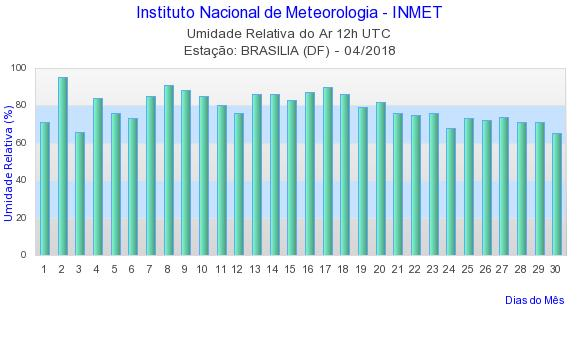
\includegraphics[width = .5 \textwidth]{sensores/figuras/sen_pc1_UR_01}
		\caption{Umidade relativa em Brasilia as 12:00 Fonte: \cite{bib_sen_03_inmet_UR}}
		\label{sen_pc1_UR_01}
	\end{figure}

	\subsection{Umidade do solo}

	A medição de umidade do solo é central para o projeto e, portanto, deve ser definida criteriosamente. Dentre as formas de medição encontradas para essa aplicação, foram separadas três categorias de sensores que cumprem as restrições de custo e disponibilidade. Esses três grupos serão avaliados em sequência e podem ser classificados em: tensiômetros, sensores resistivos e sensores capacitivos.
	
	Os tensiômetros usam um tubo a vácuo com um material poroso na ponta que permite a entrada de partículas do solo. As partículas que entram são usadas como amostras para medir o potêncial matricial da água, usando um método de sucção \cite{bib_soil_sen_emb_01}. O potencial medido pode ser então relacionado com um valor de umidade do solo. Esse sensor é normalmente encontrado em seu formato analógico porém, existem sensores digitais com princípios semelhantes, como o sensor apresentado na figura \ref{soil_sen_01}. 
	
	\begin{figure}[H]
		\centering
		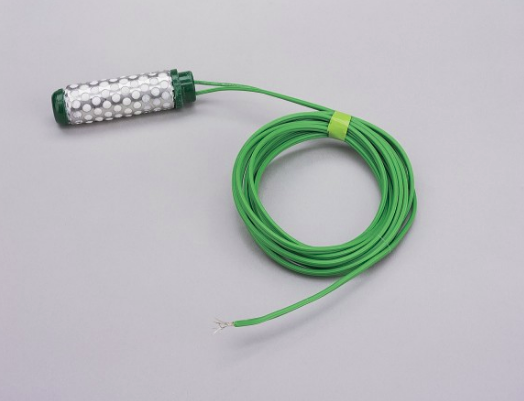
\includegraphics[width = .5 \textwidth]{sensores/figuras/soil_sen_01}
		\caption{Tensiômetro digital. Fonte: \cite{bib_soil_sen_01}}
		\label{soil_sen_01}
	\end{figure}

	A medição do potencial matricial da água por meio de tênsiometros é um método bastante usado em projetos de controle de irrigação, como por exemplo pela Embrapa \cite{bib_soil_sen_emb_02}, e, portanto, produz medições confiáveis e aceitas tanto em nível comercial quanto acadêmico. A desvantagem desse método está principalmente no preço elevado. Existem variações mais baratas desse sensor porém, não são recomendadas para uso contínuo. Além disso, o método apresenta um atraso considerável de medição (entre 77 a 90 segundos para o sensor da figura \ref{soil_sen_01}), pois depende de príncipios mecânicos de fluidos e não diretamente de variações de potenciais elétricos como nos outros sensores.
	
	Já os sensores resistivos apresentam um funcionamento mais simplificado. Esse sensor funciona por meio de dois eletrodos paralelos (figura \ref{umi_sen_res_01}), onde, uma vez inseridos, medem a resistência equivalente do solo entre eles. Como a umidade do solo influencia em sua resistência, é possível extrair um sinal proporcional a essa umidade, que pode ser calibrado para apresentar medidas mais confiáveis.
	
	\begin{figure}[H]
		\centering
		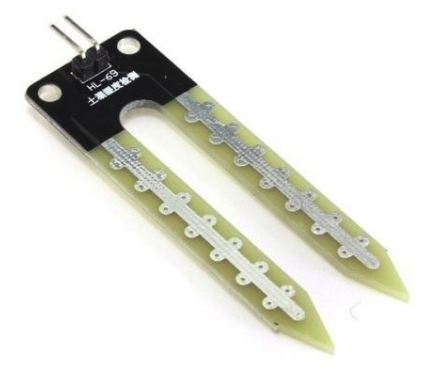
\includegraphics[width = .5 \textwidth]{sensores/figuras/umi_sen_res_01}
		\caption{Sensor de umidade resistivo. Fonte: \cite{bib_umi_sen_res_01}}
		\label{umi_sen_res_01}
	\end{figure}	
	
	A vantagem desse sensor é seu baixo preço porém, existem outros problemas que o inviabilizam para a aplicação. Primeiramente, a resistência do solo não depende exclusivamente de sua umidade mas também de outros fatores que podem prejudicar a medição. Além disso, como o sensor apresenta circuito exposto, seria necessário impermeabiliza-lo. Por último e mais importante, os eletrodos em contato com o solo oxidam rapidamente e podem se tornar inutilizáveis dentro de semanas, impossibilitando medições por longo períodos e requisitando manutenções frequentes.
	
	Por fim, os sensores capacitivos funcionam de maneira semelhante aos sensores resistivos, mas ao invés de medir uma resistência, medem uma capacitância equivalente, considerando o solo como o dielétrico. A vantagem dessa abordagem se dá em não conter eletrodos expostos e, portanto, apresentar maior durabilidade. Além disso, o sensor pode ser encapsulado, o que diminui as interferências externas e melhora a qualidade do sinal obtido.
	
	Quando comparado com o sensor resistivo, o sensor capacitivo apresenta um sinal de melhor qualidade e maior durabilidade por um pequeno aumento de custo, descartando o sensor resistivo. Apesar disso, sensores capacitivos não são comumente usados em aplicações de controle de irrigação por não apresentarem a medição mais eficiente para esse caso. Entretanto, tensiômetro digitais (disponíveis no Brasil) que permitam medições contínuas fogem do orçamento para o projeto, principalmente devido a necessidade de três sensores por estação. Alternativas mais baratas podem ser encontradas no exterior, mas o risco de entrega e custo de importação às inviabilizam para o protótipo, tendo em vista as restrições de tempo e custo do projeto.
	
	Dentre os sensores capacitivos encontrados, o que melhor se adequou ao projeto foi o sensor SoilWatch 10 da empresa Pino-Tech (figura \ref{soil_sen_03}). Esse sensor é completamente a prova d'agua e já foi usado em projetos de controle de irrigação, sendo ideal para a nossa aplicação. Suas especificação estão listadas a seguir:
	
	\begin{itemize}
				\item Custo: R\$ 85,14 
				\item Tensão de alimentação: entre $3,1V$ e $5V$
				\item Corrente de operação: $24 mA$
				\item Pinos necessários para uso: 1 (analógico)
	\end{itemize}

\begin{figure}[H]
		\centering
		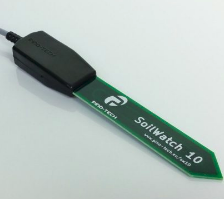
\includegraphics[width = .5 \textwidth]{sensores/figuras/soil_sen_03}
		\caption{Soil Watch 10 sensor de umidade do solo. Fonte: \cite{bib_soil_sen_03}}
		\label{soil_sen_03}
	\end{figure}	

	Entretanto, este sensor ainda não é disponível no Brasil e o custo de importação seria muito alto para o projeto, além do risco associado ao tempo de entrega. Por esse motivo, foi decidido deixar esse sensor como ideia para um produto futuro e foram avaliadas outras possibilidades mais viáveis para o protótipo. Dentre as possibilidades encontradas foi escolhido o sensor SEN0193 (figura \ref{soil_sen_02}) pelos critérios de custo e documentação disponível, já que para a maior parte dos sensores avaliados nenhuma documentação específica foi encontrada. As específicações desse sensor estão listadas a seguir.
	
	\begin{itemize}
				\item Custo: R\$ 22,00
				\item Tensão de alimentação: entre $3,3V$ e $5,5V$
				\item Corrente de operação: $5 mA$
				\item Pinos necessários para uso: 1 (analógico)
	\end{itemize}
	
	\begin{figure}[H]
		\centering
		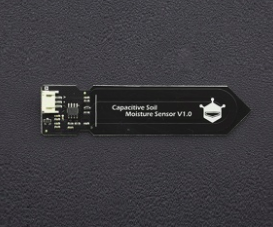
\includegraphics[width = .5 \textwidth]{sensores/figuras/soil_sen_02}
		\caption{Sensor de umidade do solo modelo SEN0193. Fonte: \cite{bib_soil_sen_02}}
		\label{soil_sen_02}
	\end{figure}	
	
	Contudo, esse sensor também não é a prova d'agua e seu circuito deve ser isolado para funcionar corretamente. Para isso, serão avaliados, futuramente, os métodos de impermeabilização mais adequados. Uma ideia inicial é o uso de époxi para cobrir o circuito.
	
	\subsection{Temperatura (solo e ar)}
		Os sensores de temperatura devem ser capazes de fazer medidas nos intervalos de temperatura esperados no ambiente e no solo brasileiros. Para as medidas que se realizarão no solo, é ainda importante que o sensor escolhido possua um encapsulamento que suporte as condições de maiores umidade e corrosividade. 
		
	O gráfico presente na figura \ref{sen_pc1_01} mostra a variação média anual da temperatura do solo no Brasil enquanto a figura \ref{sen_pc1_02} apresenta a temperatura (do ambiente) média no território brasileiro no ano de 2018. Os sensores com o propósito de medir esta grandeza mostrados a seguir contemplam estes intervalos em suas  faixas de operação.   
	
	\begin{figure}[H]
		\centering
		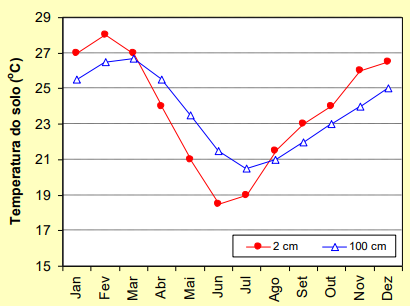
\includegraphics[width = .5 \textwidth]{sensores/figuras/sen_pc1_01}
		\caption{Media de temperatura do solo ao longo do tempo em duas diferentes profundidades. Fonte: \cite{bib_sen_02_paulo}}
		\label{sen_pc1_01}
	\end{figure}	 		

	\begin{figure}[H]
		\centering
		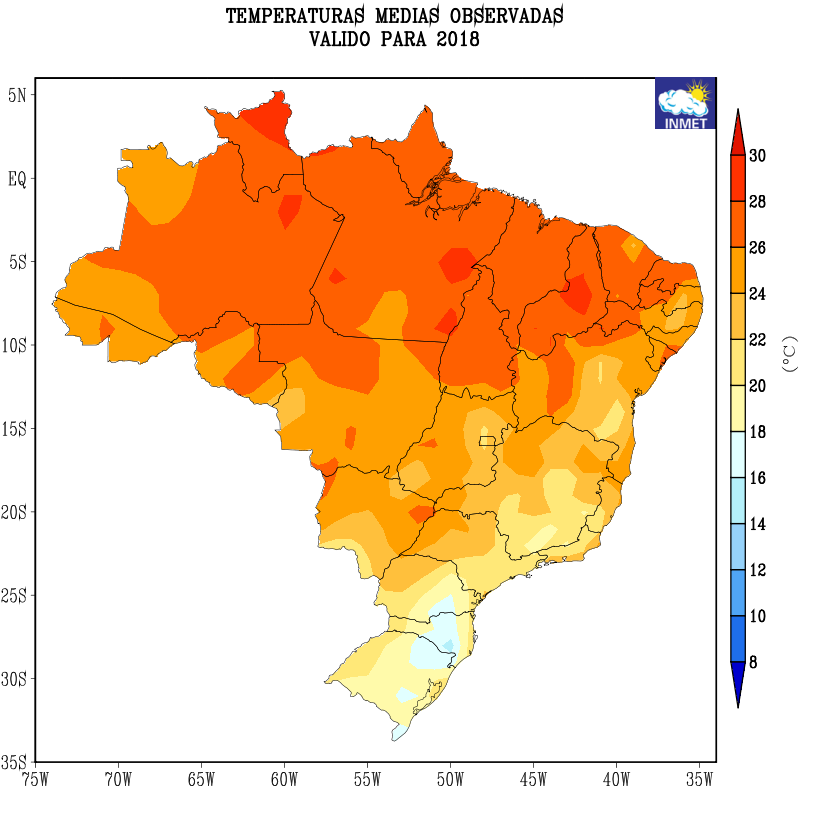
\includegraphics[width = .5 \textwidth]{sensores/figuras/sen_pc1_02}
		\caption{Temperatura média no Brasil. Fonte: \cite{bib_sen_03_inmet}}
		\label{sen_pc1_02}
	\end{figure}	 		

São vários os materiais transdutores que podem ser utilizados para medição de temperatura: termopares, termistores, termorresistências e junções PN. Abaixo estão relacionados alguns possíveis sensores comerciais que atendem as necessidades do projeto:

\begin{itemize}


	\item Temperatura ambiente:
		\begin{itemize}
			\item AM2302/DHT22: Este componente já foi apresentado como uma possibilidade de sensor para umidade do ar, mas também fornece dados relativos a temperatura ambiente. Apresenta-se como uma solução atrativa pelo fato de medir duas das grandezas necessárias. Sua acurácia para temperatura é de $\pm~0,5ºC$.  
			 
			\item LM35: Este sensor apresenta uma resposta linear em sua faixa de operação, não necessita de calibração prévia, possui baixo consumo e é de fácil utilização. Sua acurácia é de $\pm~0,5ºC$.  
			\begin{itemize}
				\item Custo: R\$ 8,91 
				\item Tensão de alimentação: entre $4V$ e $30V$
				\item Corrente de operação: $60 \mu A$
				\item Pinos necessários para uso: 1 (analógico)
			\end{itemize}

		\end{itemize}
	\item Temperatura do solo:
		\begin{itemize}
			\item Ds18b20: este é um sensor de temperatura com encapsulamento à prova d'água. Sua leitura é feita a partir de um único fio que entrega o resultado da medição em 12 bits. É um sensor de fácil utilização, mas possui acurácia de $\pm~0,5ºC$.  
			\begin{itemize}
				\item Custo: R\$ 12,99 
				\item Tensão de alimentação: entre $3V$ e $5V$
				\item Corrente de operação: $1mA$
				\item Pinos necessários para uso: 1 (digital)
			\end{itemize}
			\item Pt-100: é uma termorresistência. Geralmente, é ligado a um outro resistor formando um divisor de tensão, possui ampla faixa de operação (entre $-200ºC$ até $650ºC$) com acurácia de $\pm~0,1ºC$.
			\begin{itemize}
				\item Custo: R\$ 25,90 
				\item Tensão de alimentação: entre $3V$ e $5V$
				\item Corrente de operação: depende da resistência ligada no divisor de tensão
				\item Pinos necessários para uso: 1 (analógico) 
			\end{itemize}

		\end{itemize}

	Para o sensor de temperatura do ar será usado o módulo DHT22 por ser um sensor que também realiza a medição de umidade do ar. Já para o sensor de temperatura do solo, como a diferença de preço é baixa, será escolhido o sensor Pt-100 por apresentar uma maior acurácia.

\end{itemize}

	\subsection{Velocidade e direção do vento}

	Para simplificar o problema, as medições de velocidade e direção do vento serão reduzidas para apenas as componentes horizontais. Assim, o sistema deve medir a direção do vento como um ângulo indo de 0 a 360 graus, sendo o 0 quando o vento estiver indo em direção ao polo norte magnético e 180 ao polo sul magnético. E a velocidade do vento deve ser medida em metros por segundo e se refere a magnitude da componente horizontal do vetor de velocidade.

	O instrumento mais comum de medição da velocidade do vento é o anemômetro. Esse instrumento converte a força do vento em um movimento rotacional de um rotor, e mede a velocidade dessa rotação para estimar a velocidade do vento necessária para produzir tal movimento. Dentre o modelos de anemômetro encontrados, os anemômetros de copo destacam-se pela sua simplicidade de construções e eficiência de conversão do movimento, sua configuração se assemelha à de um gerador eólico com quatro pás no rotor, como pode ser observado na figura \ref{vel_sen_01}.
	
	\begin{figure}[H]
		\centering
		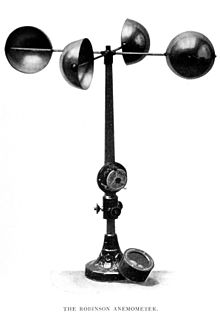
\includegraphics[width = .3 \textwidth]{sensores/figuras/vel_sen_01}
		\caption{Anemômetro de copo. Fonte: \cite{bib_vel_sen_01}}
		\label{vel_sen_01}
	\end{figure}	 		

	Levando em consideração a facilidade de construção de um anemômetro de copo, e com o intuito de reduzir os custos do projeto, foi decidido por realizar a construção desse sensor. Dessa forma, a estrutura do sensor será projetada e impressa 3D. 
	
	Para a medição de velocidade será utilizado um sensor Hall em conjunto com um imã de neodímeo preso no rotor. Como esse sensor é sensível ao campo mágnetico local, ele pode ser fixado na estrutura do anemômetro e o seu sinal pode ser processado para inferir a posição do imã. Essa configuração permite identificar quando o imã passa em cima do sensor e, consequentemente, encontrar sua velocidade. 
	
	Uma estrutura semelhante pode ser construída para realizar a medição de direção do vento. Porém, nesse caso, ao invés de usar as quatro pás utiliza-se uma haste horizontal e uma bandeira, como demonstrado na figura , de forma que a força do vento fará com que a haste se alinhe com sua direção.
	
	\begin{figure}[H]
		\centering
		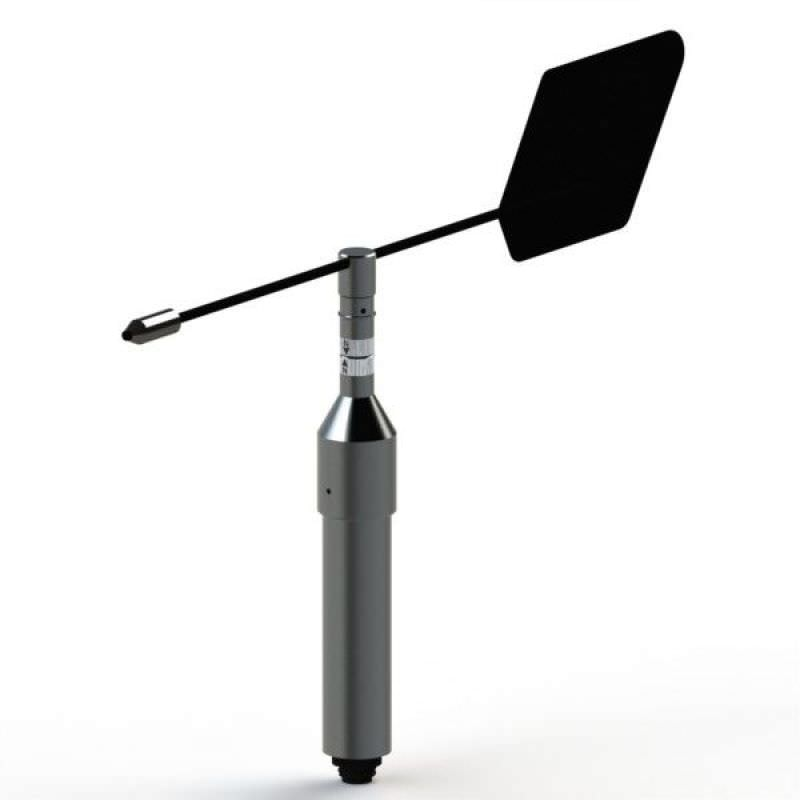
\includegraphics[width = .5 \textwidth]{sensores/figuras/dir_sen_01}
		\caption{Sensor de direção do vento. Fonte: \cite{bib_dir_sen_01}}
		\label{vel_sen_01}
	\end{figure}		
	
	Para realizar determinar a direção da haste, uma mesma configuração de sensor Hall com um imã de neodímeo será utilizada. Entretanto, como nesse caso deseja-se encontrar uma direção em ângulo, uma maior resolução espacial é necessária. Por esse motivo, serão usado quatro sensores Hall uniformemente espaçados na estrutura. Com isso, é possível processar os quatro sinais referentes às intensidades de campo magnético medidas, possibilitando uma maior acurácia na estimativa de posição.
	
	Como os requisitos de operação do sensor Hall, para essa aplicação, não introduzem muitas restrições, a escolha do sensor foi realizada apenas pelo critério de preço. O modelo do sensor escolhido é o A3144 e suas especificação estão listadas a seguir. 
	
		\begin{itemize}
				\item Tensão de alimentação: entre $5V$ e $24V$
				\item Corrente de operação: 18 mA
				\item Pinos necessários para uso: 1 (analógico) 
		\end{itemize}

	Ainda, no desenvolvimento do sensor de direção do vento, é importante que a saída seja dada em função de alguma referência fixa conhecida. Desta forma é interessante o uso de um magnetômetro no sistema. De forma análoga ao que ocorreu com o sensor de efeito Hall, os critérios de desempenho não são rígidos para a escolha do magnetômetro de forma que a escolha pode ser guiada por critérios de custo e disponibilidade. O componente escolhido foi o módulo hmc5883l, que possui as seguintes características:
		\begin{itemize}
			\item Tensão de alimentação: $3,6V$
			\item Corrente de operação: $2 \mu A$
		\end{itemize}

	\subsection{Radiação solar}

O sensor de radiação solar deve realizar as medidas de intensidade dos raios ultravioleta (UV) incidentes, gerando dados que permitam analisar sua influência no desenvolvimento da plantação. A faixa específica de radiação UV a ser medida será definida para melhor atender a variabilidade de radiação UV encontrada no território brasileiro, conforme apresentado na figura \ref{sen_pc1_03}.
		
	\begin{figure}[H]
		\centering
		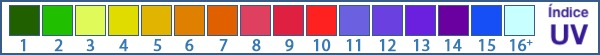
\includegraphics[width = .5 \textwidth]{sensores/figuras/sen_pc1_04}
		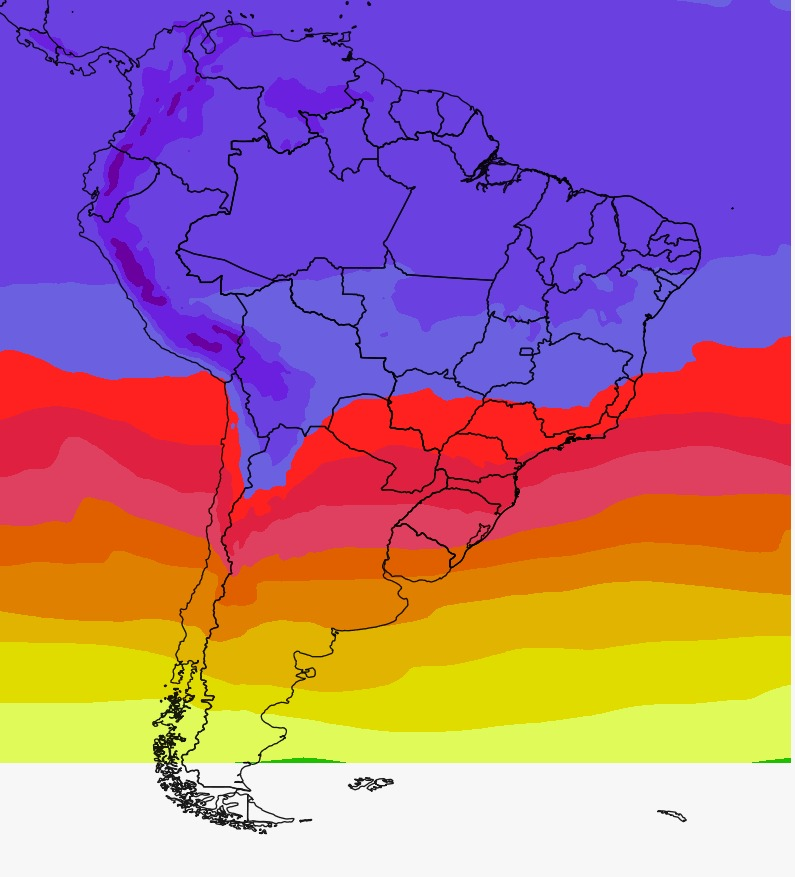
\includegraphics[width = .5 \textwidth]{sensores/figuras/sen_pc1_03}
		\caption{Nivel de intensidade UV no Brasil. Fonte: \cite{bib_sen_03}}
		\label{sen_pc1_03}
	\end{figure}

	Dentre os sensores comerciais que atendem essa faixa de operação e estão disponíveis no Brasil, foram separados duas opções, listadas a seguir.

		\begin{itemize}
			\item Ml8511: este é um sensor de raios UV com saída analógica. Por ser um sensor que possui um comportamento linear entre tensão e escala UV é possível realizar a medição diretamente com um microcontrolador já que há uma conversão interna por um amplificador operacional de foto-corrente em tensão. O sensor possui acurácia de $\pm~1UV$ nos índices definidos na escala da figura \ref{sen_pc1_03}.  
			\begin{itemize}
				\item Custo: R\$ 29,50 
				\item Tensão de alimentação: entre $3V$ e $5V$
				\item Corrente de operação: $5mA$
				\item Pinos necessários para uso: 1 (analógica)
				\item Comprimento de onda:$200\eta m-365\eta m$ 
				\item Tempo de resposta: $ ~0.5s$
			\end{itemize}
			\item UVM-30A: Possui o mesmo principio de funcionamento do sensor Ml8511 possuindo inclusive a mesma acurácia
			\begin{itemize}
				\item Custo: R\$ 80,91 
				\item Tensão de alimentação: entre $3V$ e $5V$
				\item Corrente de operação: $0,06mA$
				\item Pinos necessários para uso: 1 (analógica)
				\item Comprimento de onda:$200\eta m-365\eta m$ 
				\item Tempo de resposta: $ <0.5s$ 
			\end{itemize}

\end{itemize}

	Em ambos os sensores é necessário realizar a impermeabilização do sistema para que não haja corrosão do sensor, de forma a evitar a medição de valores inadequados. 
	
	Devido a diminuição significativa do custo, o sensor Ml8511 será escolhido para o projeto.

	\subsection{Pluviosidade}

	Existem diversas formas de medir o índice pluviométrico, ou seja, a quantidade de precipitação que incide em determinada área. Uma das formas é a utilização de um sensor de chuva (figura \ref{plu_sen_01}) que consiste em uma placa com trilhos condutivos expostos, onde sua resistência varia conforme a quantidade de água em caindo sobre sua superfície. O problema desse método é que a qualidade da medição depende de uma boa calibração do sensor e a placa em si não é a prova d'agua, necessitando de uma impermeabilização em suas conexões.
	
	\begin{figure}[H]
		\centering
		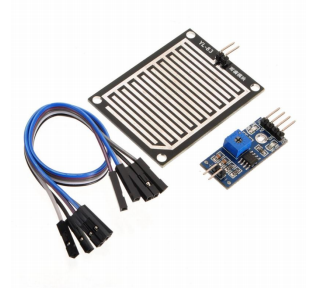
\includegraphics[width = .5 \textwidth]{sensores/figuras/plu_sen_01}
		\caption{Sensor de pluviosidade. Fonte: \cite{bib_plu_sen_01}}
		\label{plu_sen_01}
	\end{figure}
	
	Uma outra alternativa é a utilização de um sistema de balança (figura \ref{plu_sen_02}) em conjunto com um funil fechado. Nessa configuração, o funil direciona toda a precipitação incidente em sua área para o centro da balança (que vai estar tombada para um dos lados) e vai começar a encher o recipiente. Uma vez que o recipiente atinja um volume de água com peso suficiente para invertar a balança, ele será envaziado e o recipiente do outro lado passará a ser preenchido. Sabendo o volume de água necessário para essa inversão e identificando o momento em que a balança tombou, é possível determinar a quantidade de precipitação que incide na área de captação do funil em função do tempo, ou seja, o índice de pluviosidade nessa área.

	\begin{figure}[H]
		\centering
		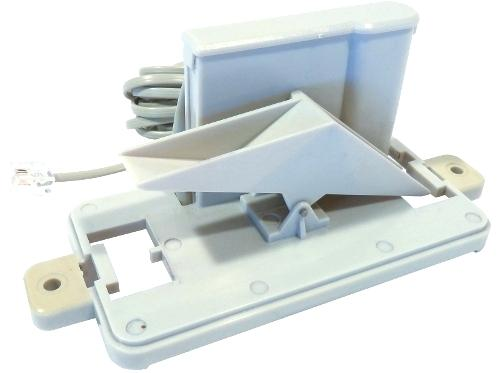
\includegraphics[width = .5 \textwidth]{sensores/figuras/plu_sen_02}
		\caption{Pluviômetro de balança. Fonte: \cite{bib_plu_sen_02}}
		\label{plu_sen_02}
	\end{figure}

	Considerando que o sistema de balança não depende de uma variação de resistência exposta (que é muito sensível à ruídos) e sim de um princípio mecânico simples, conclui-se que ele é mais robusto à interferências externas. Portanto, esse sistema foi escolhido para ser construído.
	
	A estrutura do pluviômetro de balança será impressa 3D e o mecanismo de identificação de inversão será realizado de forma semelhante aos sensores de velocidade e direção do vento. No centro da balança será fixado um imã de neodímeo e atrás da estrutura será colocado um sensor Hall deslocado para um dos lados da balança. Dessa forma, o campo magnético medido pelo sensor será maior quando a balança estiver em um dos lados do que do outro. Sabendo o valor esperado do campo magnético nas duas situações, é possível determinar para qual dos lados a balança está tombada sem a necessidade de fixar um lado inicial no ínicio da medição.
	
	Assim como nos sensores de velocidade e direção do vento, o modelo de sensor Hall a ser utilizado também será o A3114 com especificações listadas anteriormente.

	

	\subsection{pH (solo)}
	
	A acidez do meio pode ser mensurada com o auxílio de eletrodos. O valor do pH é obtido através de um valor de tensão (geralmente da ordem de milivolts) gerado nos terminais do eletrodo devido ao pH do ambiente \cite{bib_sen_06_sigel}. As características construtivas do sensor levam em consideração o meio em que será realizada a medição. Abaixo estão listadas algumas opções comerciais.
	
	\begin{itemize}
		\item Eletrodo de pH Epóxi para Semissólidos - S175CD: Este sensor tem sua faixa de operação  entre 0 e 14, sua medida não é afetada por variações de temperatura (até $100ºC$) no meio em que opera. Originalmente, foi desenvolvido para aplicações laboratoriais. 
		  
		\begin{itemize}
			\item Custo: R\$ 568,05 
			\item pinos necessários para uso: 1 (analógico) 
		\end{itemize}

		\item Eletrodo de pH HI1292D: Este é um componente desenvolvido para ser utilizado em um equipamento da própria fabricante. Assim, o sinal fornecido por este sensor já está devidamente tratado. Para que se faça o uso adequado deste eletrodo é necessário conhecer a maneira com que o sinal foi condicionado.
		\begin{itemize}
			\item Custo: informado mediando solicitação, não recebemos resposta até a entrega desde documento. 
			\item pinos necessários para uso: 1 
		\end{itemize}
		
		\item SEN-10972 (SparkFun Electronics): Este sensor não está disponível para venda no Brasil. Possui um protocolo de calibração e é vendido juntamente com o circuito para condicionar o sinal, que é fornecido em formato digital por comunicação I2C. Sua escala de operação contempla os valores de 0 a 14. As tensão e corrente informadas abaixo são referentes ao circuito de condicionamento do sinal.
		\begin{itemize}
			\item Custo: US\$ 168,75 
			\item Tensão de alimentação: $5V$
			\item Corrente de operação: $18,3 mA$
			\item pinos necessários para uso: 1 (digital) 
		\end{itemize}


	\end{itemize}
		
	Apesar de ser uma informação interessante de se fornecer ao cliente, as soluções encontradas para medição de pH são demasiadamente custosas. Esta é uma grandeza  que varia muito lentamente no tempo, de forma que o custo atual não justifica a necessidade de medições tão frequentes. Também, análises laboratoriais (comumente realizadas) são mais baratas e suficientes. Ainda serão buscadas outras metodologias de menor custo para medição da acidez do solo. Assim, a permanência desta característica do produto (capacidade de medir o pH do solo) será reavaliada. 	
	
	\subsection{GPS}
	Depois de reunidos, os dados gerados pelas estações podem ser mostrados ao usuário de diversas formas. Uma maneira interessante, que formataria as informações de maneira simples e inteligível, é a criação de uma mapa interativo. Para tanto, é necessário conhecer as posições das estações ao longo da plantação. Além de fornecer tal dado, um módulo GPS também se faz necessário para que o processo de instalação do produto seja simplificado.
	
	As opções comerciais encontradas são muito semelhantes entre si e apenas uma delas está disponível para venda por um valor mais baixo:	
	
	\begin{itemize}
		\item GPS GY-NEO6MV2: Este é um módulo de GPS projetado para ser embarcado em sistemas de baixo consumo.
			\begin{itemize}
				\item Custo: $R\$$ 65,89
				\item Tensão de alimentação: $3,6V$
				\item Corrente de operação: $100 mA$
			\end{itemize}
	\end{itemize}
	
\begin{figure}[H]
	\centering
	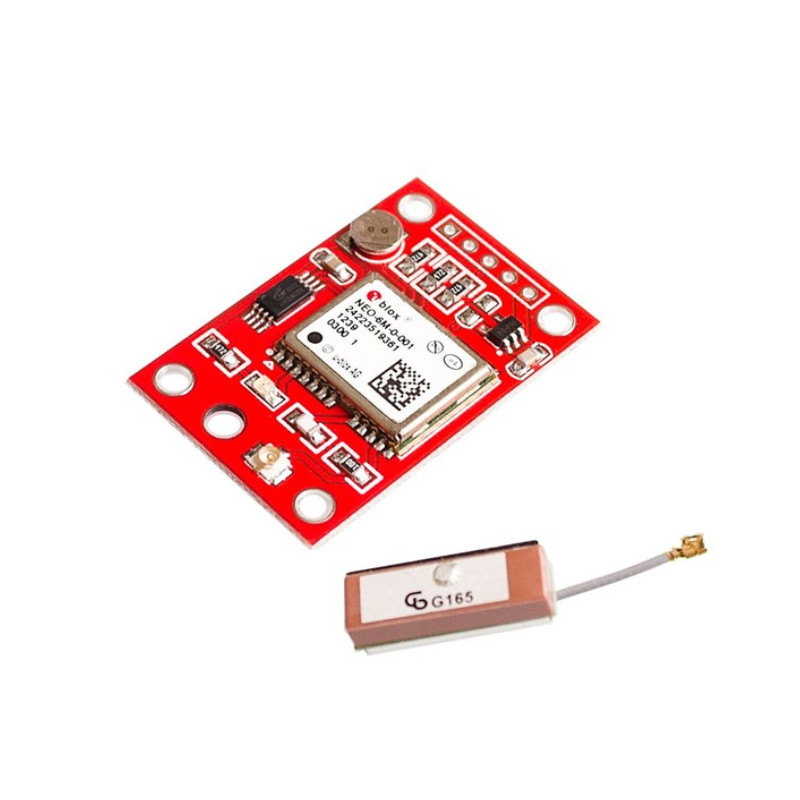
\includegraphics[width = .4 \textwidth]{sensores/figuras/sen_pc1_05}
	\caption{Módulo GPS GY-NEO6MV2. Fonte: \cite{bib_sen_pc1_10}}
\end{figure}	

	
	
\section{Processamento de Sinais}
	Os dados coletados em cada um dos sensores devem ser tratados e interpretados para que se consiga gerar informações significantes ao usuário e comandos para o controle automatizado da irrigação. Nas estações, os sinais gerados nos sensores devem ser devidamente condicionados e armazenados para que sejam enviados para a central, que reunirá as informações de todas as estações da rede e enviará comando para os atuadores. Para cada um dos componentes do sistema, estão elencadas abaixo as características desejadas no contexto do processamento de dados:
	
	
		\begin{itemize}
			\item Estações:
				\begin{itemize}
					\item Condicionar adequadamente os sinais dos sensores
					\item Armazenar os dados gerados por no mínimo 12 horas
					\item Possibilitar a implementação da rede com as demais estações
					\item Baixo consumo de energia		
				\end{itemize}
			\item Central:
				\begin{itemize}
					\item Reunir os dados de todas as estações
					\item Enviar os dados para o servidor em nuvem
					\item Gerar os sinais de comando para os atuadores
				\end{itemize}
			\item Atuador:
			\begin{itemize}
				\item Interpretar adequadamente os sinais recebidos e executar a ação desejada (ligar ou desligar a irrigação)
				\item Sinalizar se o comando solicitado pode ou não ser executado 
				\item Baixo consumo de energia
			\end{itemize}				
		\end{itemize}		 

	\subsection{Escolha do hardware}
	Como visto anteriormente, cada uma das partes do sistema possui características específicas para seu funcionamento. Por este motivo, a escolha do hardware será tratada individualmente para cada uma delas. As possibilidades avaliadas são microcontroladores, sistemas operacionais embarcados e computadores pessoais. 
		
		\begin{itemize}
			\item Estações: aqui será realizada a aquisição e o processamento dos sinais de todos os sensores. Além disso, também serão implementados os protocolos e algoritmos de comunicação para formação de uma rede. Tendo em vista a complexidade e quantidade de processos necessários, as funcionalidades de um sistema operacional mostram-se mais adequados dentre as opções mencionadas. Tanto um sistema embarcado quanto um computador pessoal atendem as demandas de processamento requeridas. Entretanto, dada a necessidade de baixo consumo e as limitações espaciais da estrutura, um sistema operacional embarcado mostra-se como melhor opção.   
			
			\item Central: este componente é responsável por gerenciar todo fluxo de informações produzido pelas estações e enviar tais dados a um servidor em nuvem. Novamente, os computadores e sistemas operacionais são as melhores opções dentre as levantadas. Considerando que esses dados serão apresentados ao usuário apenas pela aplicação externa, o sistema na central não requer uma interface gráfica nem um monitor. Levando em conta também os gastos energéticos e o custo, sistemas embarcados são mais apropriados nesse caso.
			
			\item Atuador: O controle dos atuadores são as tarefas mais simples (em termos computacionais) realizadas pelo sistema e não demandam as ferramentas oferecidas por um sistema operacional. Logo, além de possuir baixo consumo energético, um microcontrolador supre as necessidades deste módulo. 
				
		\end{itemize}
		
O projeto, então, demandará os seguintes componentes para processamento de sinais: um microcontrolador para o módulo Atuador e duas placas com sistema operacional embarcado para a Central e para Estação. Estes componentes foram escolhidos levando em consideração sua disponibilidade entre os membros com o objetivo de reduzir os custos do grupo com prototipagem. Abaixo estão listados os componentes escolhidos e suas características:
 
		
\begin{itemize}
\item msp430g2553:
    \begin{itemize}
		\item Custo: $R\$ 29,90$
		\item Processador:16-Bit RISC Architecture
		\item Memoria RAM : 1GB LPDDR2 SDRAM
		\item Tensão de alimentação: $3,3V$
		\item Corrente de operação:$230 \mu A$ (modo ativo)	
		\item Pinos disponíveis: 16 (leitura GPIO)
	\end{itemize}
\item Raspberry Pi 3 model B: É um single board computer (SBC), um sistema embarcado que simula um computador em uma unica placa, sendo então parte do seu sistema saídas digitais, processador, memoria ram. 
	\begin{itemize}
		\item Custo: $R\$ 179,90$
		\item Processador: Broadcom BCM2837B0, Cortex-A53 64-bit SoC @ 1.4GHz
		\item Memoria RAM : 1GB LPDDR2 SDRAM
		\item Tensão de alimentação: $5V$
		\item Corrente de operação:$0,6 A$	
		\item Pinos disponíveis: 40 (leitura GPIO)
		\item Dispositivos de comunicacão: 2.4GHz e 5GHz IEEE 802.11.b/g/n/ac wireless LAN, Bluetooth 4.2, BLE. Gigabit Ethernet acima de USB 2.0 (rendimento máximo de 300 Mbps)
    \end{itemize}
\end{itemize}				  		
	\subsection{Condicionamento dos sinais}
	
	Nesta etapa serão analisados os sinais gerados pela estação e como eles devem ser condicionados para entrar na Raspberry Pi. A partir das informações especificadas anteriormente, definimos os seguintes sinais gerados:
	
	\begin{itemize}
			\item Umidade do ar / Temperatura do ar: 2 sinais digitais
			\item Velocidade e direção do vento: 5 sinais analógicos
			\item Radiação solar (UV): 1 sinal analógico
			\item Pluviosidade: 1 sinal analógico
			\item Umidade do solo: 3 sinal analógico
			\item pH: indeterminado
			\item Temperatura do solo: 1 sinal analógico
			\item GPS: 2 pinos digitais (comunicação serial)
			\item Bússola: 2 pinos digitais (comunicação I2C)
	\end{itemize}
	
	Assim, serão 11 sinais analógicos, 2 sinais digitais de uso comum, 2 sinais digitais seriais TX/RX e 2 sinais digitais seriais SCL/SDA. A placa Raspberry Pi definida já possui entradas GPIO, TX/RX e SCL/SDA, portanto, nesses casos, a conexão é direta. Para os sinais analógicos será necessário o uso de conversores A/D.
	
	Dentre os conversores A/D encontrados, foi separado por critério de custo o modelo ADS1115 de 16 bits, que conta com quatro entradas analógicas. Suas especificações estão listadas a seguir.
	
	\begin{itemize}
		\item Custo: $R\$ 29,40$
		\item Tensão de alimentação: $2 - 5.5V$
		\item Corrente de operação:$150 \mu A$
		\item Pinos disponíveis: 4 analógicos
		\item Comunicação: serial I2C
	\end{itemize}
	
	Assim, serão necessários 3 conversores A/D desse modelo e eles se conectarão à placa por meio dos terminais I2C e usando as portas SCL e SDA.
	
	